\documentclass{beamer}
\usetheme{Madrid}
 
\usepackage[utf8]{inputenc}

\usepackage{amsmath}
\usepackage{amsfonts}
\usepackage{array}

\usepackage{graphicx}
\graphicspath{{./figs/}}
\usepackage{subfigure}
\usepackage{multirow}
\usepackage{xspace}


\usepackage{tikz}
\usetikzlibrary{arrows, shapes, positioning}

\newtheorem*{remark}{Remark}

%Information to be included in the title page:
\title{Robustness of Transaction Ledgers}

\author{Runchao Han}
\institute{}
\date{}

\begin{document}

\frame{\titlepage}

%%%%%%%%%%%%%%%%%%%%%%%%%%%%%%%%%%%%%%%%%%%%%%%%%%%%%%%%%%%%%%%%%%%%%%%%%%%%%%%%%%%%%%%%%%%%%%%%

\begin{frame}
\frametitle{Overview}

\begin{itemize}
    \item Nakamoto consensus maintains a public transaction ledger.
    \item Public transaction ledger: A ``book'' recording transactions.
\end{itemize}

\begin{figure}
    \centering
    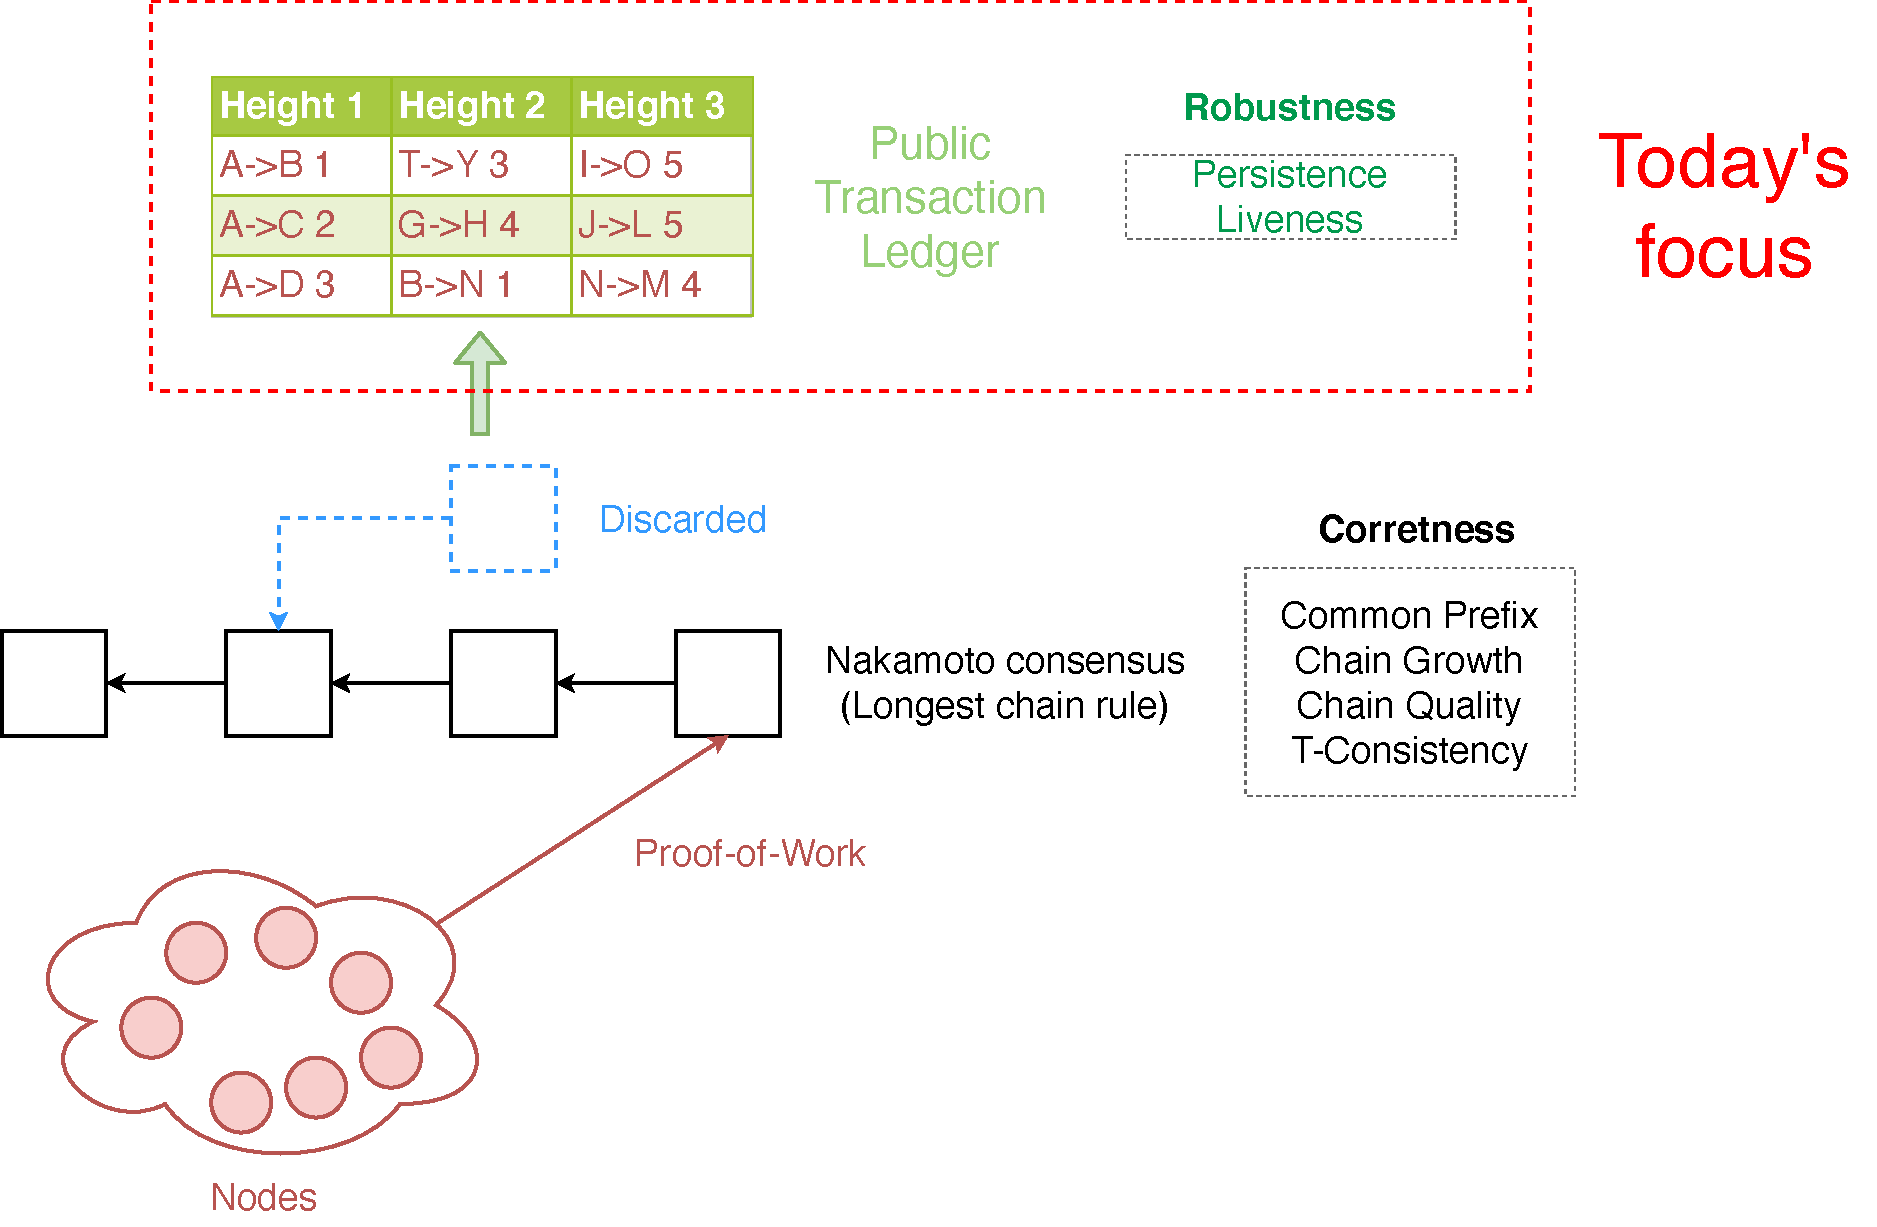
\includegraphics[width=.8\textwidth]{overview.pdf}
\end{figure}

\end{frame}


\begin{frame}
\frametitle{Model}

Chain, ledger, transaction, account\dots

\begin{itemize}
    \item A public transaction ledger is a set of transaction ledgers $\mathcal{L}$ and a set of transactions $\mathcal{T}$.
    \item Each miner maintains a chain $\mathcal{C}$, which contains a ledger $\mathsf{x}_{\mathcal{C}}$.
    \item A ledger $\mathsf{x} \in \mathcal{L}$ is a vector of sequences (blocks) $\langle x_1, x_2, \dots, x_m \rangle$.
    \item Each sequence $x$ consists of transactions of the form $x = \langle tx_1, tx_2, \dots, tx_e \rangle \in \mathcal{T}$.
    \item Each transaction $tx$ may be associated with one or more accounts, denoted as $a_1, a_2, \dots$.
\end{itemize}

\end{frame}


\begin{frame}
\frametitle{Transactions}

\begin{itemize}
    \item $C(tx_1, tx_2) = 1$ means two transactions $tx_1$ and $tx_2$ are \emph{conflicting}.
    \item A transaction $tx$ is \emph{neutral} if $C(tx, tx') = 0$ for any other $tx'$.
    \item Transactions are generated by calling the $\mathsf{Txgen}(\cdot)$ oracle.
    \item We say $\mathsf{Txgen}(\cdot)$ is \emph{unambiguous} if for all PPT $\mathcal{A}$,
        \[
            Pr \left[ C(tx, tx') = 1
            \begin{array}{|c}
                tx \gets \mathsf{Txgen}(\cdot)\\
                tx' \gets \mathcal{A}^{\mathsf{Txgen}}(\cdot)
            \end{array}
            \right] = \kappa
        \]
    \item the probability that $\mathcal{A}^{\mathsf{Txgen}}$ produces a transaction $tx'$ s.t. $C(tx, tx')$ for any $tx$ issued by $\mathsf{Txgen}(\cdot)$ is negligible in $\kappa$.
\end{itemize}

\end{frame}


\begin{frame}
\frametitle{Robustness of a Public Transaction Ledger}

\begin{itemize}
    \item \textbf{Persistence}: once an honest miner reports a tx ``deep enough'' in the ledger, all other honest miners will report it at exactly the same position.
    \item \textbf{Liveness}: neutral txs will be inserted in the ledger within a sufficient number of rounds.
\end{itemize}

\begin{definition}[Robust transaction ledger]
    A protocol $\Pi$ implements a \emph{robust transaction ledger} in the $q$-bounded synchronous setting if it satisfies \emph{Persistence} and \emph{Liveness}.
\end{definition}

\end{frame}



\begin{frame}
\frametitle{Persistence}

\begin{definition}[Persistence]
    Parametrised by $k \in \mathbb{N}$ (the ``depth'' parameter). If in a certain round an honest player reports a ledger that contains a transaction $tx$ in a block more than $k$ blocks away from the end of the ledger, then $tx$ will always be reported in the same position in the ledger by any honest player from this round on.
\end{definition}

\begin{remark}[The depth parameter $k$]
    After $k$ blocks, a block is considered ``stable'', i.e., can be reverted with negligible probability.
    The negligible function takes $k$ as one of its parameters.
    In Bitcoin, the value of $k$ is 6 (recommended by the community).
\end{remark}

\end{frame}


\begin{frame}
\frametitle{A Ledger without Persistence over Correct Nakamoto Consensus}

\begin{itemize}
    \item The accumulator does not preserve orders of txs.
    \item The hash of accumulators of two blocks is same.
    \item Anyone can manipulate the order of transactions in a block.
\end{itemize}

\begin{figure}
    \centering
    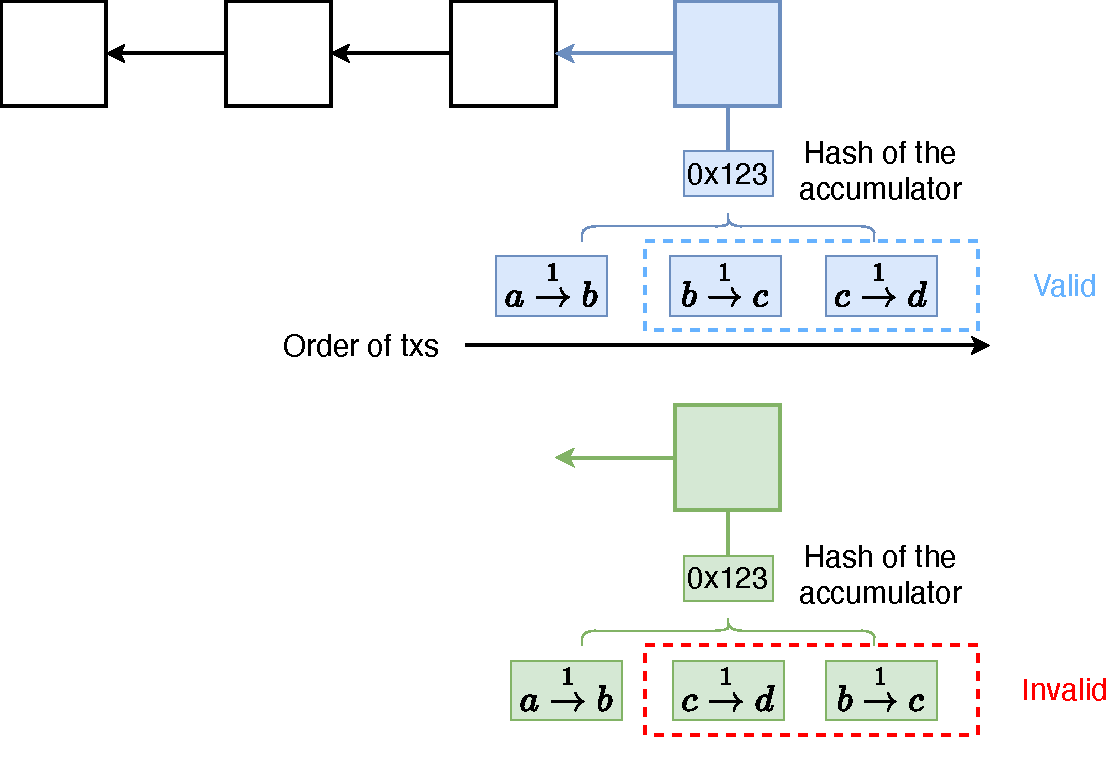
\includegraphics[width=.6\textwidth]{no-persistence.pdf}
\end{figure}

\end{frame}


\begin{frame}
\frametitle{Liveness}

\begin{definition}[Liveness]
    Parametrised by $u, k \in \mathbb{N}$ (the ``wait time'' and ``depth'' parameters, resp.). Provided that a transaction either (i) issued by $\mathsf{Txgen}$, or (ii) is \emph{neutral}, is given as input to all honest players continuously for $u$ consecutive rounds, then there exists an honest party who will report this transaction at a block more than k blocks from the end of the ledger.
\end{definition}

\begin{remark}[An informal rephrase]
    Once a valid transaction is submitted, it should become $k$-``stable'' within $u$ new blocks.
\end{remark}

\end{frame}


\begin{frame}
\frametitle{A Ledger without Liveness over Correct Nakamoto Consensus - Case 1}
    
A transaction takes $>= u-k$ blocks to be included.

\begin{figure}
    \centering
    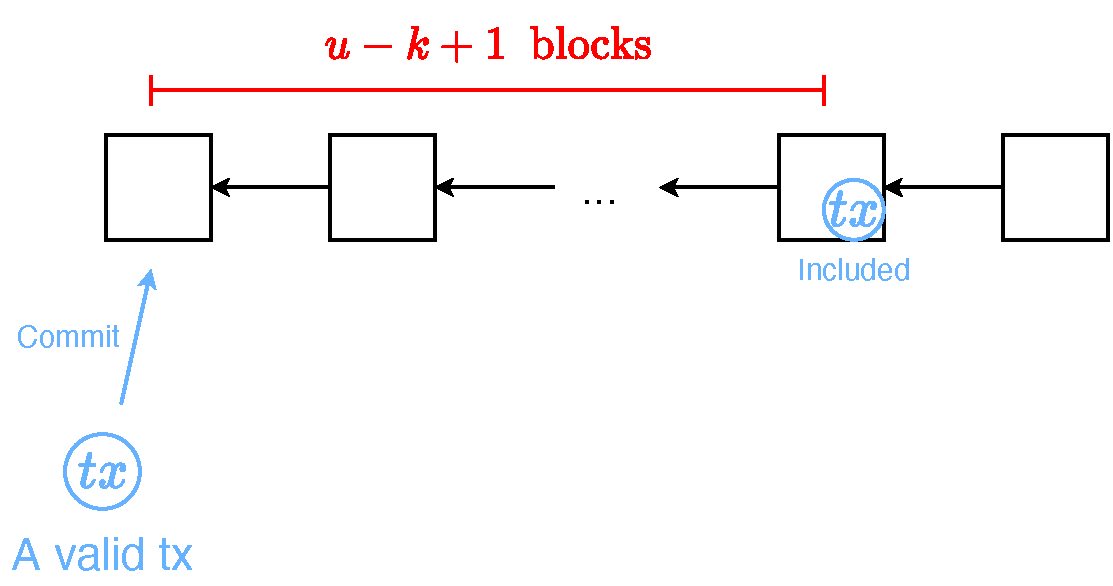
\includegraphics[width=.6\textwidth]{no-liveness-1.pdf}
\end{figure}

\end{frame}


\begin{frame}
\frametitle{A Ledger without Liveness over Correct Nakamoto Consensus - Case 2}
    
A transaction takes $< u-k$ blocks to be included, but later reverted by a longer fork.

\begin{figure}
    \centering
    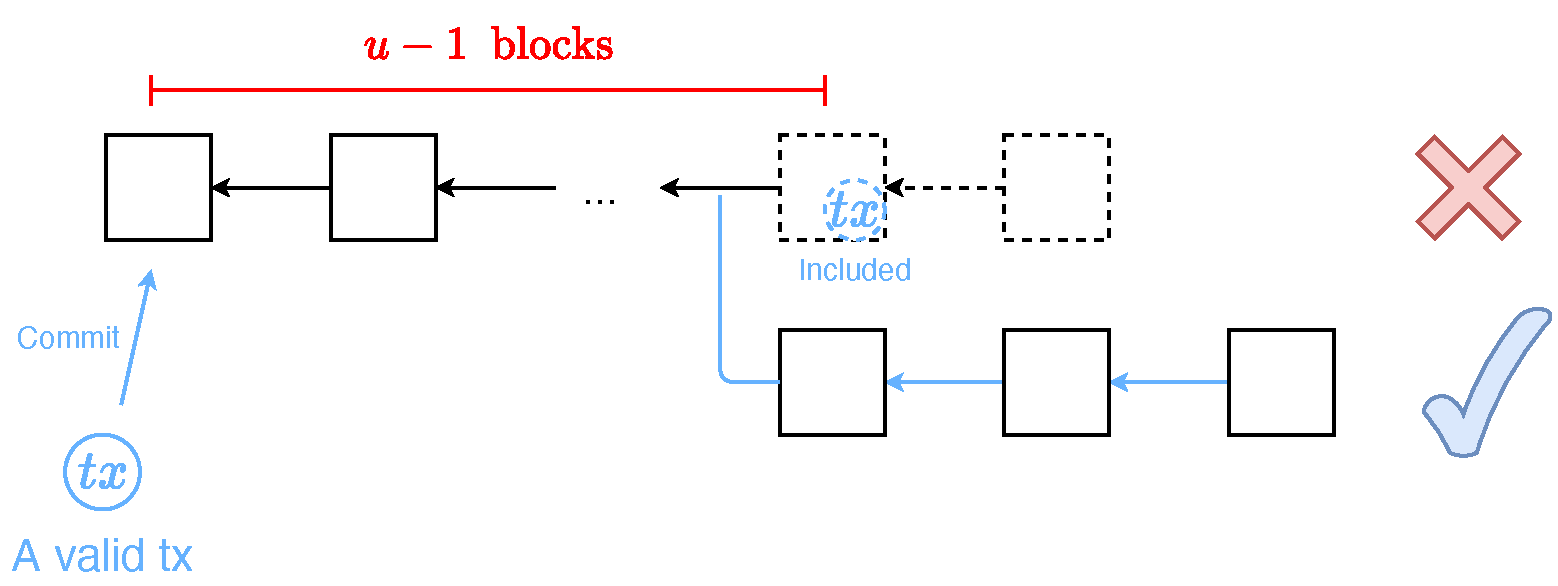
\includegraphics[width=.6\textwidth]{no-liveness-2.pdf}
\end{figure}

\end{frame}

\begin{frame}
\frametitle{Proving Persistence and Liveness - Notations}

\begin{itemize}
    \item $n, t$ is \# of miners/Byzantine miners.
    \item $\{0, 1\}^\kappa$ is the range of a hash $H(\cdot)$.
    \item $D$ is the difficulty parameter.
    \item $p = \frac{D}{2^\kappa}$ is the success rate of a hash.
    \item $q$ is \# of hashes a miner can do in a round.
    \item $\alpha = pq(n-t), \beta = pqt, f = \alpha + \beta$ is \# of solutions honest/malicious/all miners can find in a round, resp.
\end{itemize}

\end{frame}


\begin{frame}
\frametitle{Two lower bounds}

The parameter $\gamma = \alpha - \alpha^2$ is a lower bound on two possibilities:
\begin{itemize}
    \item At least one honest miner computes a solution in a round
    \begin{align}
        Pr &= 1 - (1-p)^{q(n-t)}\\
           &= 1 - (1-p)^{\frac{\alpha}{p}}\\
           &= 1 - [(1-p)^{\frac{1}{p}}]^\alpha\\
           &\geq 1 - e^\alpha \geq \alpha - \alpha^2 = \gamma
    \end{align}
    \item Exactly one honest miner computes a solution in a round
    \begin{align}
        Pr &= {q(n-t) \choose 1} p(1-p)^{q(n-t)-1}\\
           &= (n-t)qp(1-p)^{q(n-t)-1}\\
           &= \alpha (1-p)^{q(n-t)-1}\\
           &\geq \alpha (1-\alpha+p) \geq \gamma
    \end{align}
\end{itemize}

\end{frame}



\begin{frame}
\frametitle{Theorems}

\begin{theorem}[Persistence]
    Suppose $f < 1$ and $\gamma \geq (1 + \delta)\lambda \beta$ for some real $\delta \in (0,1)$ and $\lambda \geq 1$ such that $\lambda^2 - f\lambda - 1 \geq 0$.
    Protocol $\Pi_{\mathsf{PL}}$ satisfies \emph{Persistence} with probability $1 - e^{\Omega(\delta^3k)}$, where $k$ is the depth parameter.
\end{theorem}

\begin{theorem}[Liveness]
    Suppose $f < 1$ and $\gamma \geq (1 + \delta)\lambda \beta$ for some real $\delta \in (0,1)$, $\lambda \in [1, \infty)$ and let $k \in \mathbb{N}$.
    Further, assume $\mathsf{Txgen}$ is \emph{unambiguous}.
    Protocol $\Pi_{\mathsf{PL}}$ satisfies \emph{Liveness} with wait time $u = \frac{2k}{(1-\delta)\gamma}$ and depth parameter $k$ probability $1 - e^{\Omega(\delta^2k)}$.
\end{theorem}

Proofs rely on previous lemmas on CP, CG, CQ, \dots

\end{frame}


\begin{frame}[allowframebreaks]
    \frametitle{References}
    \bibliographystyle{alpha}
    \tiny\bibliography{refs}
\end{frame}

\end{document}